\documentclass[tikz,border=8pt]{standalone}
\usetikzlibrary{arrows.meta,positioning,circuits.ee.IEC}
\begin{document}
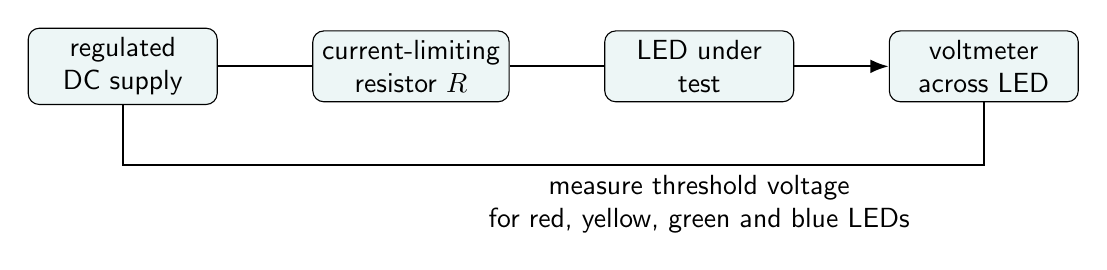
\begin{tikzpicture}[font=\sffamily,>=Latex,box/.style={draw,rounded corners,minimum height=9mm,minimum width=24mm,align=center,fill=teal!7}]
\node[box] (supply) {regulated\\DC supply};
\node[box,right=12mm of supply] (res) {current-limiting\\resistor $R$};
\node[box,right=12mm of res] (led) {LED under\\test};
\node[box,right=12mm of led] (meter) {voltmeter\\across LED};
\draw[thick,-Latex] (supply)--(res)--(led)--(meter);
\draw[thick] (meter.south)--++(0,-8mm)-|(supply.south);
\node[below=8mm of led,align=center] {measure threshold voltage\\for red, yellow, green and blue LEDs};
\end{tikzpicture}
\end{document}
